%
% File acl2012.tex
%
% Contact: Maggie Li (cswjli@comp.polyu.edu.hk), Michael White (mwhite@ling.osu.edu)
%%
%% Based on the style files for ACL2008 by Joakim Nivre and Noah Smith
%% and that of ACL2010 by Jing-Shin Chang and Philipp Koehn


% % Notes -

% % Change Abstract with the latest methods and results


% %
% %


\documentclass[10pt]{article}
\usepackage{acl2012}
\usepackage{times}
\usepackage{latexsym}
\usepackage{amsmath}
\usepackage{multirow}
\usepackage{url}
\usepackage{verbatim}


% my packages

\usepackage{algorithm}
\usepackage{amsmath}
\usepackage[noend]{algpseudocode}
\usepackage{amsfonts,amssymb}
\usepackage{program}
\usepackage{graphicx,amssymb,amsmath}
\usepackage[english]{babel}
\usepackage{listings}
\usepackage[official]{eurosym}
\usepackage{caption}
\usepackage{subfig}


\newcommand*{\argmin}{\operatornamewithlimits{argmin}\limits}
\newcommand*{\argmax}{\operatornamewithlimits{argmax}\limits}

\iffalse
\DeclareMathOperator*{\argmax}{arg\,max}
\setlength\titlebox{6.5cm}    % Expanding the titlebox
\fi

\title{Inference in Graphical Models - Crowdsourcing Problem}

\author{
  Pavankumar Reddy M , Kiran Koshy T \\
  {\tt muddire2@illinois.edu}, {\tt thekump2@illinois.edu}  \\
  Department of Electrical and Computer Engineering \\
  University of Illinois at Urbana-Champaign \\}

\date{May 4, 2015}

\begin{document}
\maketitle
\begin{abstract}
  This paper discusses designing an inference algorithms for a crowdsourcing problem given noisy responses from possibly unreliable workers, under the Dawid-Skense model. The objective is to minimize the average error probability with a fixed budget constraint on how many task-worker pairs can be assigned to get responses on.
  
\end{abstract}

\section{Introduction}

Crowdsourcing problem involves estimating the correct answers for a set of tasks given the responses from a set of workers  each of whom responded to a subset of these tasks. In this paper, tasks are assumed to be binary and are produced according to a prior distribution which is bernoulli with a label of a task being,

\begin{equation}
t_i = \left\{
\begin{array}{cc}
+1~~\text{with probability 3/4}\\
-1~~\text{with probability 1/4}
\end{array}
\right. \label{eq:t_prior}
\end{equation}

The objective here is to estimate the task labels as $\hat{t}_i$ so that the error probability is

$$P_e(\hat{t}) = \frac{1}{n}\sum\limits_{i = 1}^{n}\mathbb{P}(t_i\ne \hat{t_i}),$$

is minimized.

In this paper, the label for the $i^{th}$ task would be denoted by $t_i$ and reliability of $j^{th}$ worker is denoted by $p_j$. The response given by the $j^{th}$ worker for the $i^{th}$ task would be denoted by $A_{ij}$.

The main method adopted to achieve this is Expectation Maximization. A little introduction to belief propagation is given at the beginning although the method was not pursued because of the time limitations for this project.

\subsection{Belief Propagation}

The joint likelihood for tasks labels denoted by $t_i$ (of task $i$) and reliability parameters for worker denoted by $p_j$ (of worker $j$) given responses $A_{ij}$ (to task $i$ by worker $j$) is denoted by $\mu(t,p\vert A)$ and assuming the generative model assumed for the project, it would be,
$$\mu(t,p\vert A) \propto \mu(t,p,A) \propto \mu(A\vert t,p)\mu(t)\mu(p)$$
$$\mu(t,p\vert A) = \frac{1}{Z}\prod_{i\in [n]}{F'(t_i)}\prod_{j\in [m]}{F(p_j)}\prod_{(i,j)\in E}\psi_{ij}(A_{ij},p_j,t_j)$$
where, $$\psi_{ij}(A_{ij}, p_j, t_j) = \mathbb{I}(t_i=A_{ij})p_j + \mathbb{I}(t_i=-A_{ij})(1-p_j)$$

Here $F'(t_i)$ is the bernoulli (0.75) prior of task labels shown above and $F(p_j)$ is the beta distribution with $\alpha = 6$ and $\beta = 2$.\\

From this joint distribution one could derive the updates for messages in the Belief Propagation algorithm. But, the message from workers to tasks would involve sending a continuous distribution and messages from tasks to workers would involve integrating over it. Both these aspects are difficult to overcome as is. So, workers reliabilities are limited to a finite support and the summation over this finite support would be equivalent to approximate numerical integration. In our case, the support is generated by quantizing the beta distribution to $10$ samples between $0$ and $1$ with $3$ in $0$ to $0.5$ and $7$ in the remaining to adjust for the rightward bias of the beta distribution with the given parameters of $\alpha$ and $\beta$. The messaging passing updates are derived to be as follows,\\
  	Messages from worker to task,
  	$$\nu_{j\rightarrow i}(p_j)\propto\prod_{k\in \partial j\setminus i}\sum_{t_k}F'(t_k)\psi_{kj}(t_k, p_j)\nu_{k\rightarrow j}(t_k).$$
  	Messages from task to workers,
  	$$\nu_{i\rightarrow j}(t_i)\propto\prod_{k\in \partial i\setminus j}\sum_{p_k}\bar{F}(p_k)\psi_{kj}(t_i, p_k)\nu_{k\rightarrow i}(p_k),$$
 
where $\bar{F}(p_j)$ is the discretized version of the beta distribution $F(p_j)$ .
 
 We wrote this belief propagation in \textit{python} utilizing \textit{networkx} library which helped us implement the graphical model as a graph data structure. With this approach an error rate of $<0.005$ was achieved for a budget of $nl = 30000$ which is $5$ times the required error rate. Since this belief propagation approach was taking close to $1$ hour to just do $3-4$ iterations we decided against building the adaptive algorithm on top of it. Thus we moved our focus to expectation maximization.
 
\subsection{Expectation Maximization} \label{init}
The expectation maximization could be performed on maximizing the likelihood of the observations $A$ given parameters. So, EM could be run with either $t$ or $p$ as parameters. In this paper, the EM algorithm is limited to treating $p$ as parameters with $t$ as a hidden variable in the likelihood equation. The likelihood equation looks like the one shown in the earlier section. The objective here would be,
$$p* = \argmax_p\mu_p(A) = \argmax_p\sum_{t\in\{-1,+1\}^n}\mu_p(t,A)$$
where, $$\mu_p(t,A) = \frac{1}{Z}\prod_{i\in [n]}{F'(t_i)}\prod_{(i,j)\in E}\psi_{p_j}(A_{ij},t_j)$$

The first stage of the EM algorithm or E-step boils down to calculating the conditional distribution $\mu_p(t\vert A)$ of the task labels $t$ given the observation $A$ and the current estimate $p$ of the parameter. This would be,
 $$\mu_p(t\vert A) = \frac{1}{Z}\prod_{i\in [n]}{F'(t_i)}\prod_{(i,j)\in E}\psi_{p_j}(A_{ij},t_j)$$
 where, $$\psi_{p_j}(A_{ij}, t_j) = \mathbb{I}(t_i=A_{ij})p_j + \mathbb{I}(t_i=-A_{ij})(1-p_j).$$
 
Note that $\mu_p(t\vert A))$ can be written as the product,
$$\mu_p(t\vert A) = \prod q_i(t_i \vert A_{i \partial i}),$$ where $q_i(\cdot)$ is the marginal conditional distribution of the task label $t_i$ given its neighbours $\partial i$. $q_i(\cdot)$'s are initialized to fraction of positive and negative responses for task $i$ which is just majority voting.

In the second step of the Expectation Maximization or the M-step we estimate the worker reliability parameter $p$ which maximizes the expected value of the likelihood function conditioned over the distribution $\mu_p(t \vert A)$ obtained in the E-step. This optimum value of the reliability parameter of worker $j$ would be,
$$p_j = \frac{\sum_{i\in \partial j}q(A_{ij})}{\vert\partial j\vert}.$$

The update equations for one round of EM would would be,
 
$$q_i(t_i) \leftarrow \frac{F'(t_i)\prod_{j\in \partial i} \mu_{p_j}(A_{ij}\vert t_i)}{\sum_{t'_i\in {-1,+1}}F'(t'_i)\prod_{j\in \partial i} \mu_{p_j}(A_{ij}\vert t'_i)},$$
$$p_j \leftarrow \frac{\sum_{i\in \partial j}q(A_{ij})}{\vert\partial j\vert}.$$

\section{Basic EM}

\subsection{Basic EM Task Assignment} \label{task-assign}
Given a number of tasks and workers with $l$ and $r$ parameters, Erd\H{o}s-R\'enyi is not used, rather a random $(l, r)$ graph is generated by taking $nl$ half edges and $mr$ half edges and connecting a random permutation of them. Note that multiple edges between the same nodes are merged into one single edege. This ensures that the degree distribution is uniform  across both tasks and workers instead of bernoulli as in Erd\H{o}s-R\'enyi graph. So, when running the basic EM this approach for task assignment is used. The task assignment for adaptive version of the algorithm is described later.

\subsection{Observations}
Its been observed that number of workers for a given budget should not be of the order of the number of tasks. For the case of $l= 15$, the plot of error with number of workers is shown below in Figure. \ref{error_num_workers}. As one can observe, the number of workers, for ideal results, is an order less than the number of tasks. This could be explained by the fact that, as the number of workers decrease, the fanout ($r$) of each worker increases, increasing the accuracy of their reliability estimates.

			
\begin{figure}[h!]
	\centering
	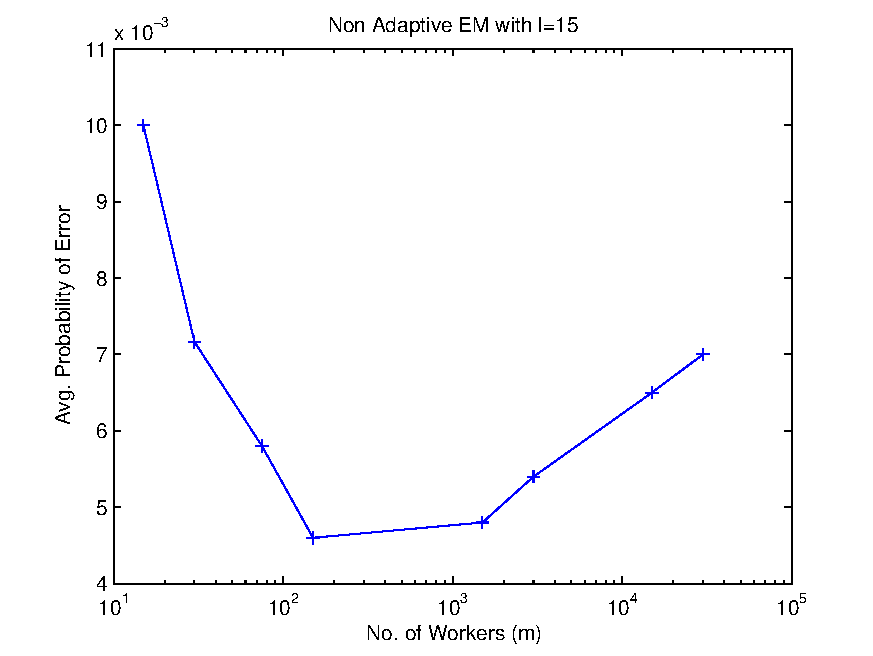
\includegraphics[width=0.5\textwidth]{worker_error.pdf}
	\caption{The plot of error with number of workers}
	\label{error_num_workers}
\end{figure}

Here we define the quality of estimate of task labels as, $\vert q_i(+1) - q_i(-1) \vert$. With this definition of quality, one can expect it to be an indicator of how confident an estimate of task label, $i$ is. As expected, the average quality of miss-classified labels was lower than correctly classified labels. But most interestingly we found that the difference in these average qualities (between miss-classified and correctly classified labels) was increased significantly as the number of workers increased. The plot of the same is shown in Figure. \ref{quality_plot}. This may be because of the fact that as the number of workers decreases, the parameter $p_j$ of each worker $j$ is estimated with higher accuracy and this in turn leads to the fact that only the tasks with all mostly uncertain workers would be miss-classified.
			
\begin{figure}[h!]
	\centering
	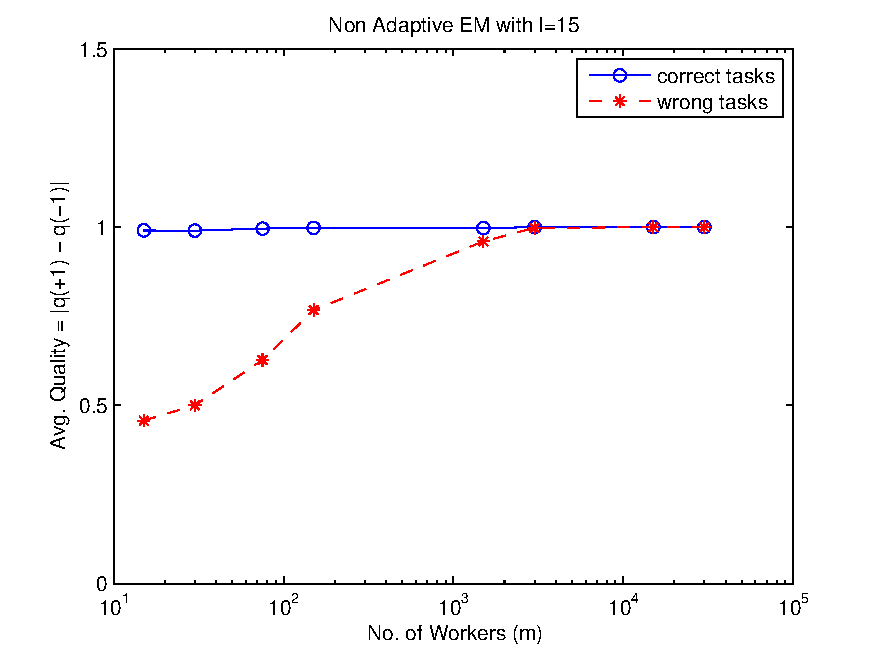
\includegraphics[width=0.5\textwidth]{quality_diff2.pdf}
	\caption{The plot of quality with number of workers}
	\label{quality_plot}
\end{figure}

So, the adaptation could be done on assigning more workers to these low quality tasks. The adapted algorithm with this stategy is discussed in the next section. Additionally, a similar metric for workers would be $\vert2p_j - 1 \vert$ which indicates how good a worker is. Unlike previously defined quality for workers which indicates how bad the estimate of task label is, this assumes that the estimated $p_j$ is good estimate and defines whether a worker is good at predicting the label. Observe that workers who tell the truth ($p_j$ near $1$) or lie ($p_j$ near $0$) are beneficial for out EM algorithm. So, one could imagine that removing the ``bad" workers and increasing the quality of task label estimates. But, its been observed that the task estimates are very sensitive to the number of workers and reduction of workers after their $p_j$ estimates severely affect the performance of the whole algorithm. So, this particular path of adaptation was abandoned.

\section{Adapted EM algorithm}

\subsection{Algorithm}
\begin{itemize}
\item[0.]
Let remaining budget $B$, be initialized as $nl_0$, where $l_0$ be the given budget parameter. Also set $n'=n$. Let the set of tasks be $T$. Let the set of workers be initialized to $P = \phi$. Finally the set of selected tasks is initialized to $T'=\phi$.
\item[1.]
If $B/n$ is less than one stop the algorithm. Let current useful budget be $b = B/2$. Now $l = b/n'$ and $m = 2b/n'$.
\item[2.]
Assimilate a set of $m$ new workers $P'$, with work reliability parameters and add it to $P$.
\item[3.]
Now similar to the basic EM we add $b$ more edges between the selected vertex set $T'$ of tasks and the selected set of workers $P'$ according to section Section \ref{task-assign}.
\item[4.]
Run the basic EM algorithm on graph with vertices as $(T, P)$ and the $q_i(\cdot)$ initialized with the results from the previous run of EM. If this is the first round the initialization of $q_i(\cdot)$ is initialized using majority voting as mentioned in Section \ref{init}.
\item[5.]
Set selected vertex set $T'=\phi$. First rank the tasks according to the ascending value of their quality and add the bottom half of the tasks to $T'$. Next rank the tasks according to ascending order of their degree and then add bottom $1/100$-th of the tasks to $T'$.
\item[6.]
Now set $n' = \|T'\|$, cardinality of selected vertex set. Reduce the budget by the number of edges added in the previous run of EM $B = B - b$.
\item[7.]
Goto step 1.
\end{itemize}



\subsection{Summary}

In summary the we run every run of EM with half the current available budget of users and accordingly assimilate new workers. Also each run of EM is started by initializing the values of the $q_i(\cdot)$ as the result from the previous round.

Also at end of each iteration we selected set of the tasks with low quality and low number of edges and assign new workers only to these tasks.


\subsection{Observations}

As seen in the earlier plain EM, keeping the number of workers in the order of number of tasks was non-ideal. This was again observed in adapted EM.
This could primarily be because $p_j$ estimate needs a large $r$ which intern implies a small $m$ for a given budget $n\times l$. The ideal estimates were observed when $m = l$ or $m = 2l$. The adapted EM with more workers just for low quality workers was not giving some outliers with good quality but an incorrect estimate of label. Its been seen that degree of such nodes was low. (We start out with uniform degree but it changes as more wokers are added to some of the tasks). So, low degree tasks are also provided with more workers.
    					
\subsection{Results}

The final mean error is $3.33\times 10^{-4}$ for $m = l$ and $2\times 10^{-4}$ for $m = 2l$. 
\begin{figure}%
	\centering
	\subfloat[The plot of error with $l$]{{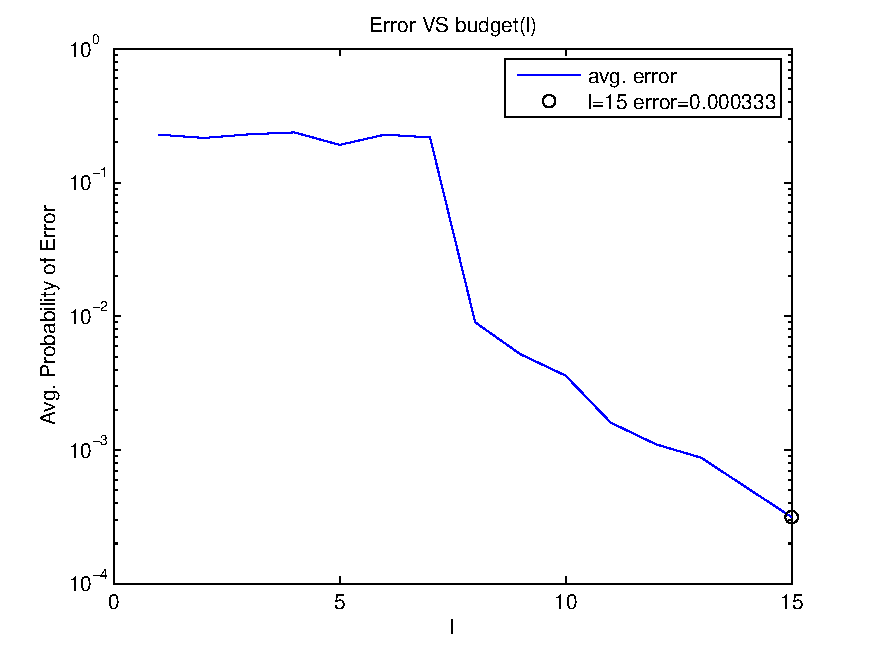
\includegraphics[width=0.5\textwidth]{avg_error1.pdf} }}%
	%\qquad
	%\subfloat[Sample 2]{{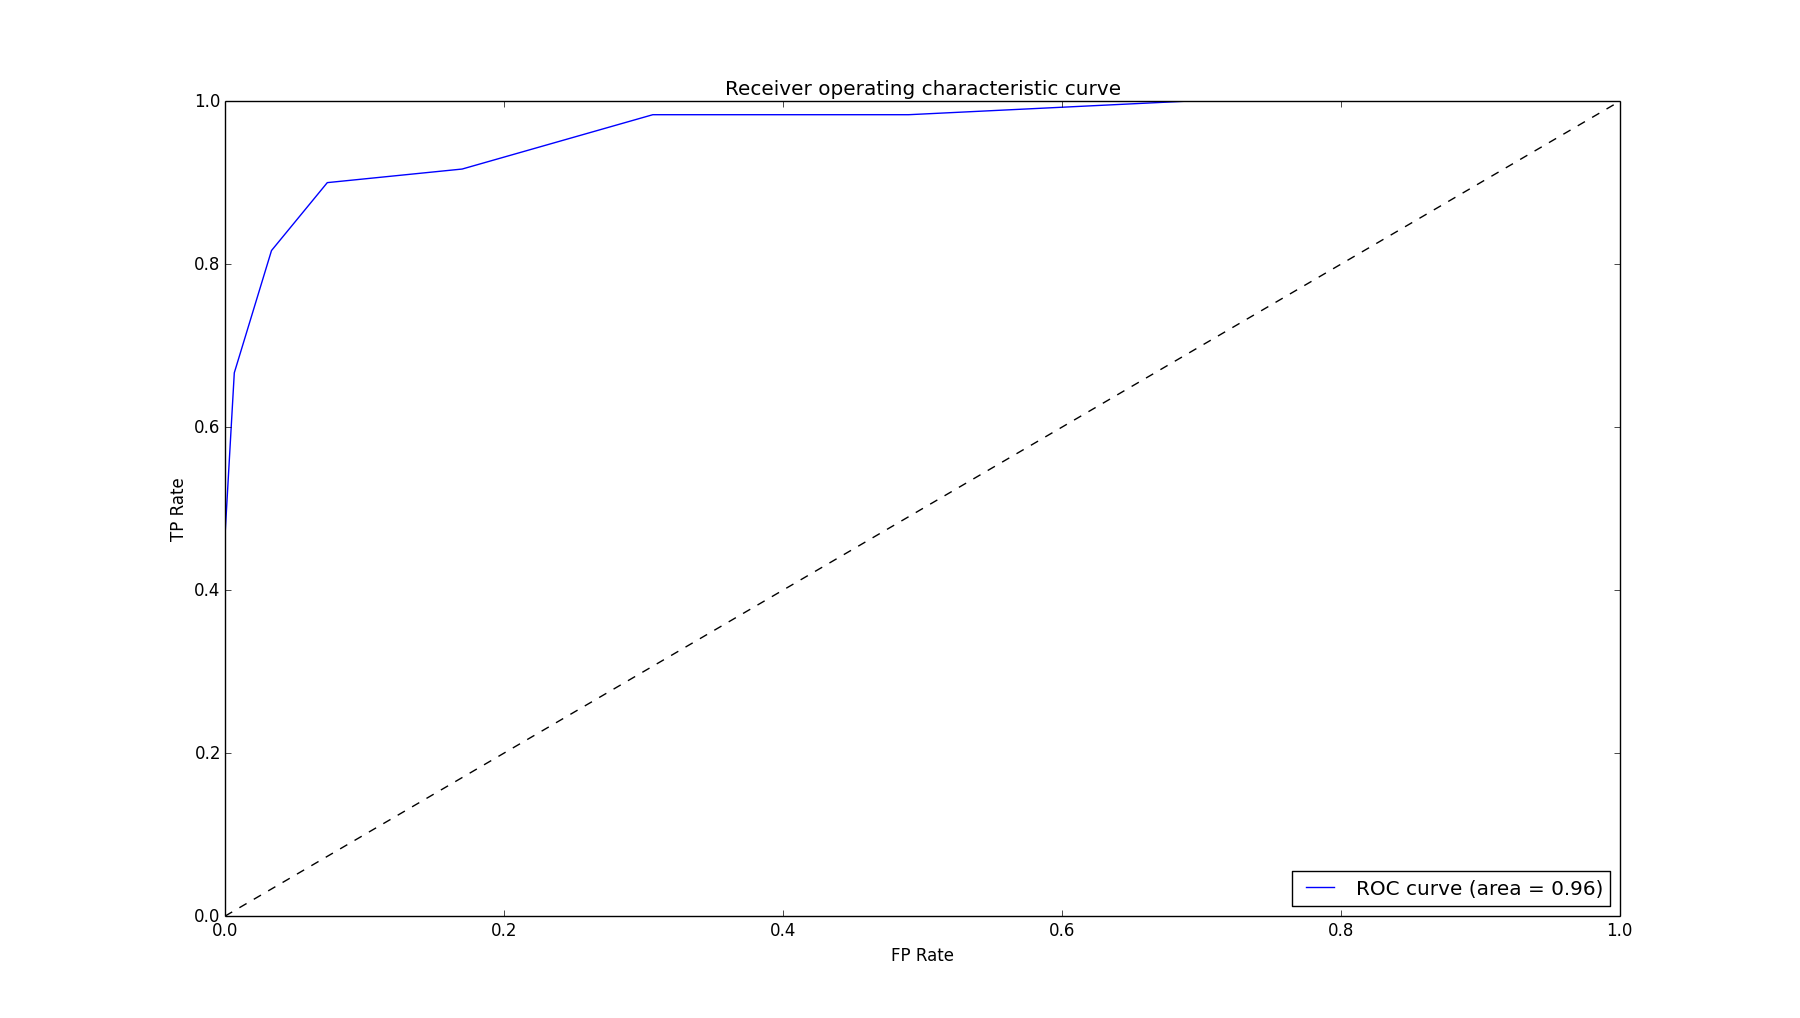
\includegraphics[width=0.5\textwidth]{roc4} }}%
	\qquad
	\subfloat[The plot of error with $l$, ]{{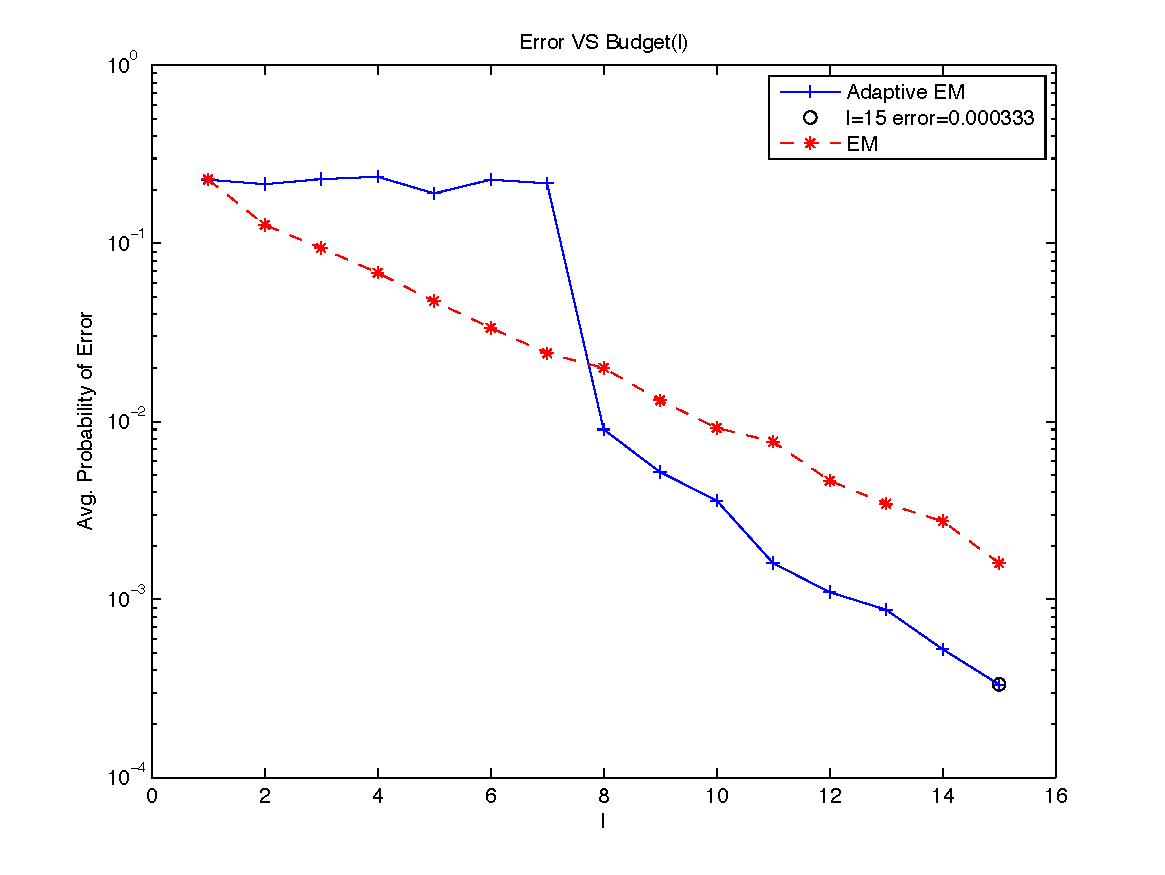
\includegraphics[width=0.5\textwidth]{avg_error2.pdf} }}%
	%\qquad
	%\subfloat[Sample 4]{{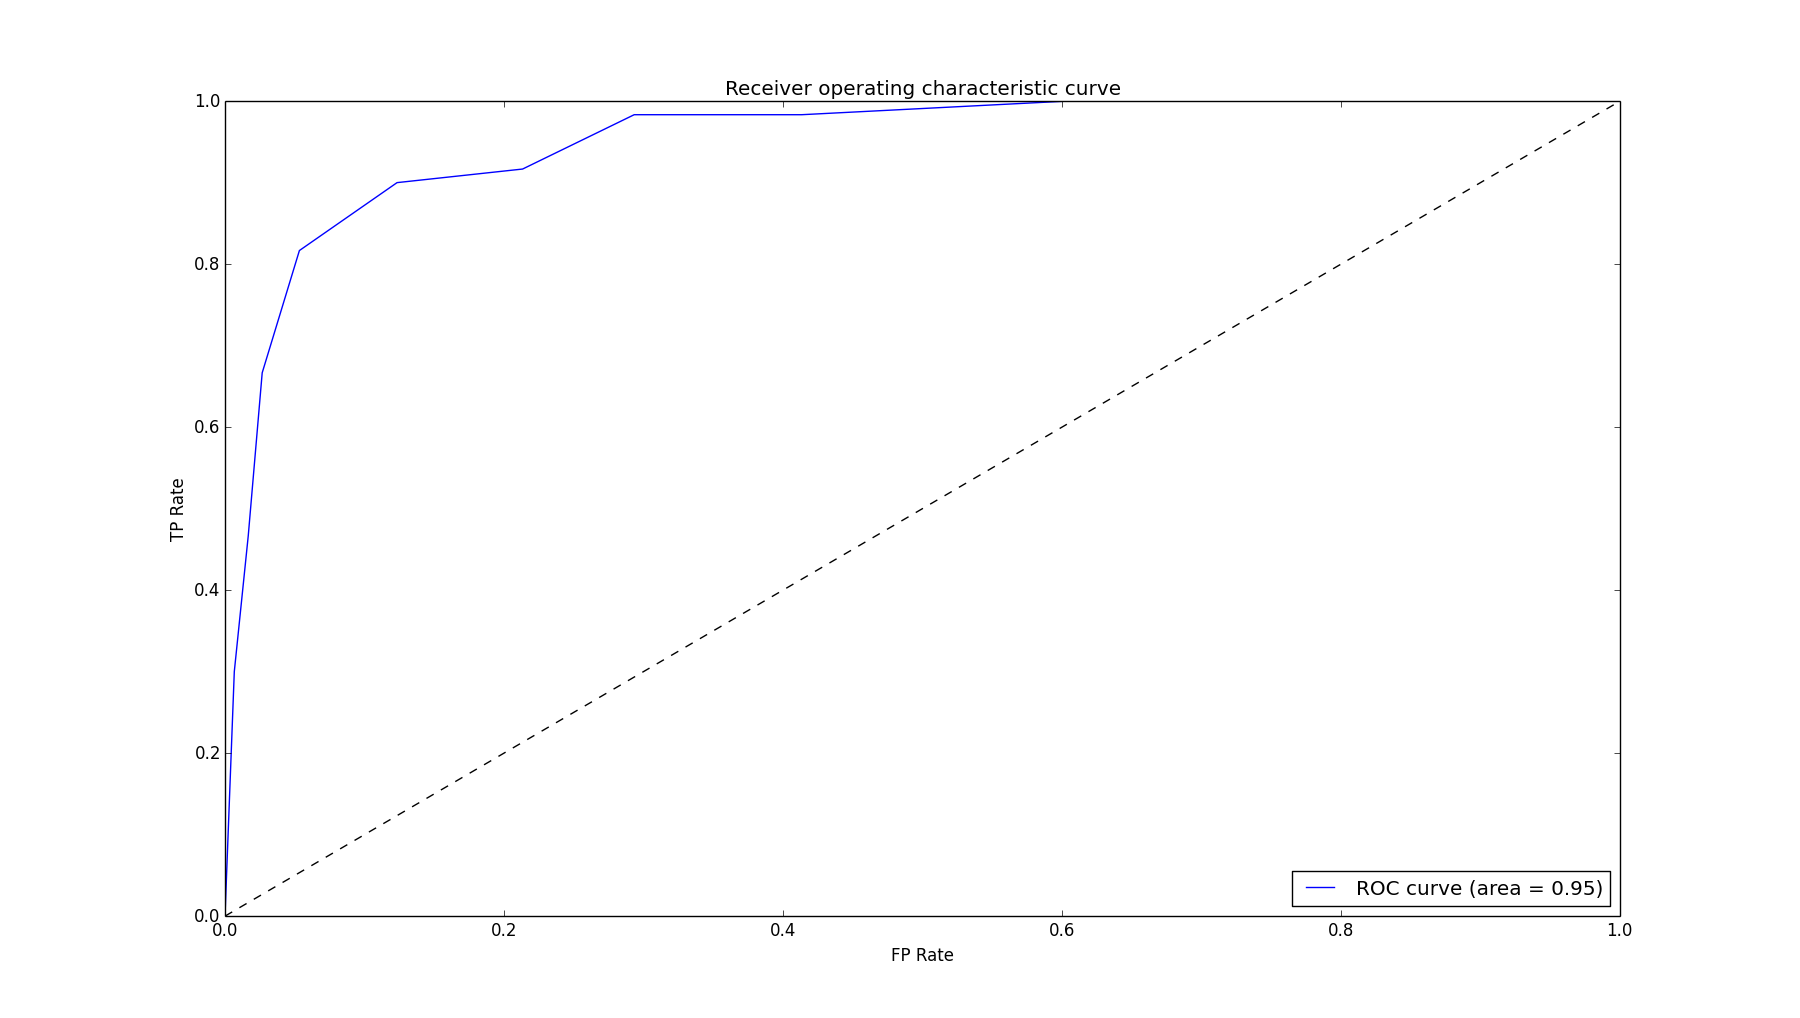
\includegraphics[width=0.5\textwidth]{roc2} }}%
	%\qquad
	%\subfloat[Sample 5]{{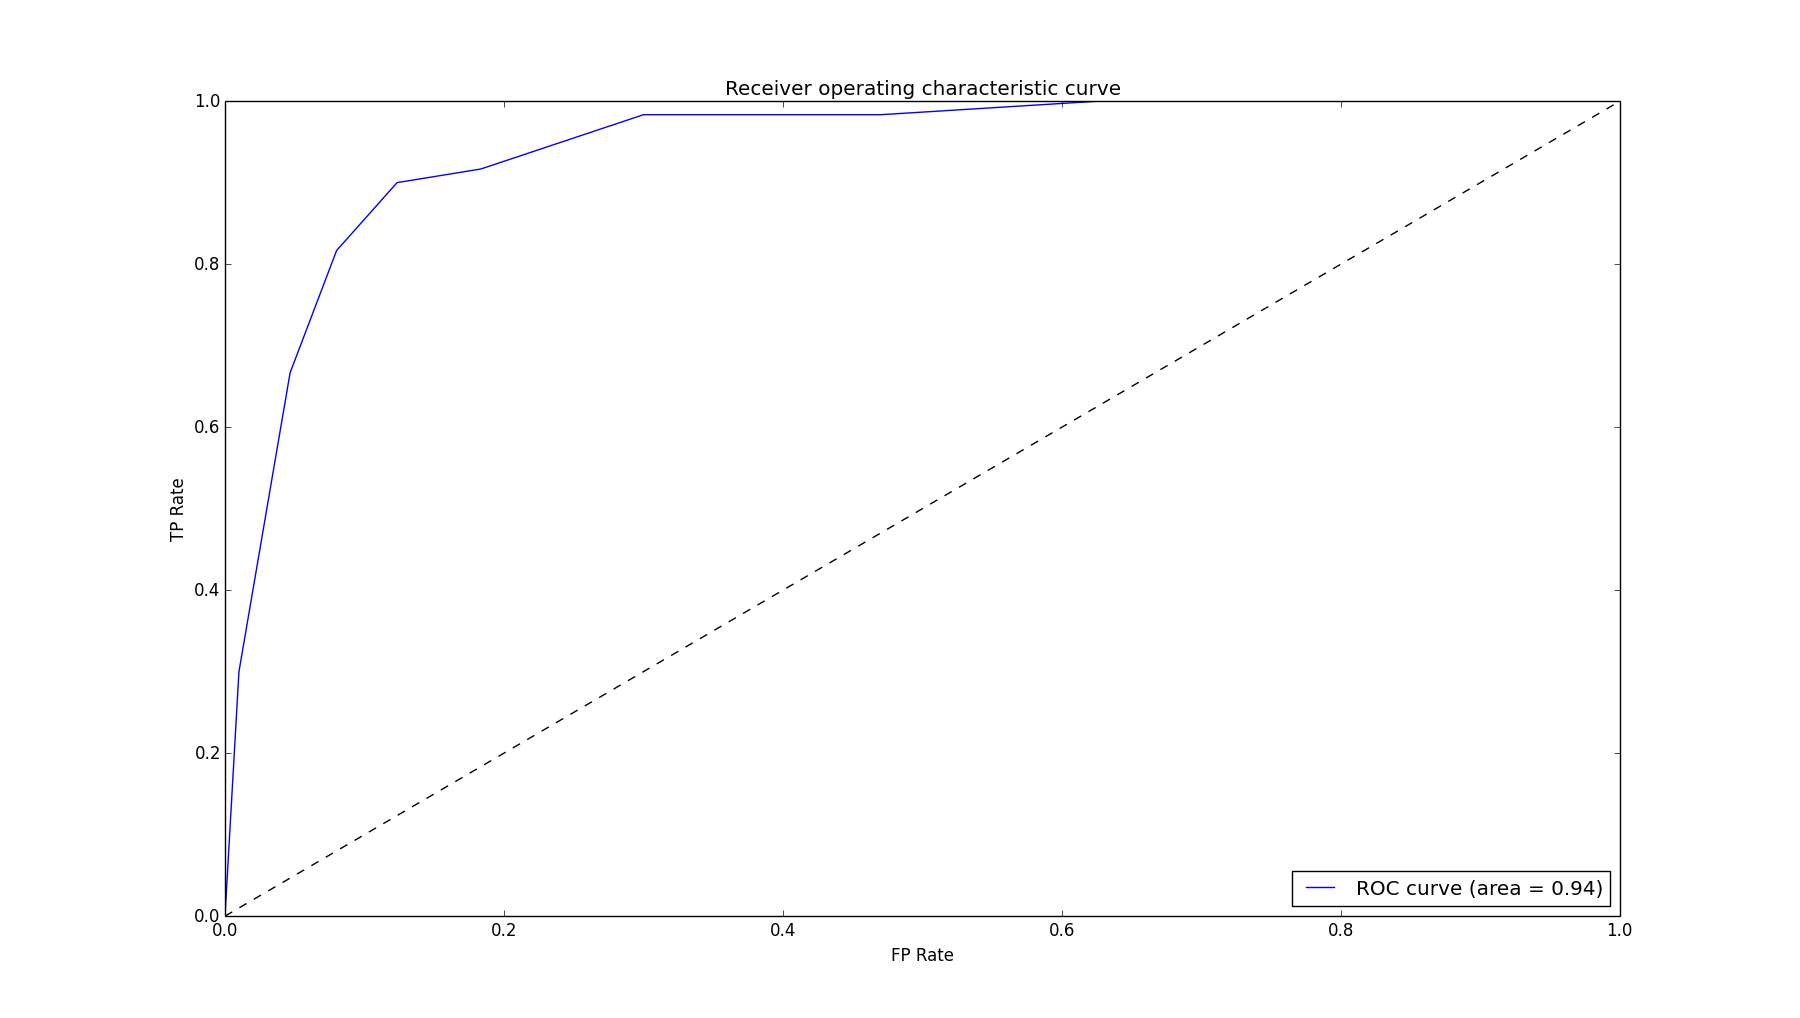
\includegraphics[width=0.5\textwidth]{roc5} }}%
	\caption{Final Curves}%
	\label{fig:final}%
\end{figure}



\begin{thebibliography}{}


\bibitem[\protect\citename{}2014]{Aho:72}
David R. Karger and
Sewoong Oh and
Devavrat Shah
\newblock 2011.
\newblock {\em Budget-Optimal Task Allocation for Reliable Crowdsourcing Systems}.
\newblock abs/1110.3564

\bibitem[\protect\citename{variational}]{citekey}
Liu, Qiang and Jian Peng and Ihler, Alex T
\newblock 2012
\newblock {\em Variational Inference for Crowdsourcing}
\newblock {Advances in Neural Information Processing Systems 25}, 692--700

\end{thebibliography}

\end{document}
